\section{Simulation Results and Discussion}\label{sec:results}

Unless noted otherwise, all inferential comparisons span $N=10$ paired random seeds ($100\text{--}109$). Because $p = 2/2^{10} \approx 0.002$ ($0.00195$) is the minimum attainable two-sided exact paired Wilcoxon signed-rank $p$-value for $N=10$ whenever all 10 seed pairs agree in sign (rank-biserial correlation $|r_{\text{rb}}| = 1.000$), I report paired mean differences ($\Delta$), Student-$t$ 95\% confidence intervals, rank-biserial $r_{\text{rb}}$, and paired Cohen's $d_z$ alongside exact $p$-values (full paired statistics appear in the online supplement).

\subsection{E1: Multi-Region Cluster Carbon--SLO Frontier}\label{subsec:res_e1}
Table~\ref{tab:e1_results} and Fig.~\ref{fig:e1_pareto} summarize \texttt{E1} across 1h and 24h horizons. On conversational traffic (\texttt{conv}), hybrid routing \texttt{P4} lowers $\text{SCI}_{\text{op}}$ by 60.77\% at 1h ($\Delta = -0.05124$ [-0.05473, -0.04775] g/1k tok, $r_{\text{rb}} = -1.000$, $d_z = -10.50$, $p = 0.002$) and 60.70\% at 24h ($\Delta = -0.04948$ [-0.05220, -0.04676], $d_z = -13.01$, $p = 0.002$) relative to carbon-agnostic colocation \texttt{B1}, and by 43.95\%--44.07\% relative to intra-region phase disaggregation \texttt{B2} ($d_z \in [-19.99, -11.29]$, $p = 0.002$). Because fixed hardware amortization adds $\text{SCI}_{\text{emb}} \approx 0.0090$~gCO$_2$eq/1k tok across equal-capacity clusters, total $\text{SCI}_{\text{tot}}$ drops 54.92\% (1h) and 54.64\% (24h) versus \texttt{B1} at 0.81\%--0.82\% SLO violations (TTFT P95 = 504.5--506.4~ms), well below the 5\% boundary.

By contrast, unconditional spatial disaggregation \texttt{P3} reaches lower $\text{SCI}_{\text{tot}}$ (0.03858 at 24h) at the cost of tail degradation, breaching 5\% at 24h (5.90\% violations, TTFT P95 = 1,190.4~ms). \texttt{P4} cuts \texttt{P3} SLO violations by 83.57\% (1h, $\Delta = -4.12\text{ pp}$ [-5.12, -3.11]) and 86.04\% (24h, $\Delta = -5.08\text{ pp}$ [-6.16, -4.00], $r_{\text{rb}} = -1.000$, $p = 0.002$) for a +6.48\%--6.79\% $\text{SCI}_{\text{tot}}$ trade-off, supporting \textbf{H1} and \textbf{H2}.

\begin{figure*}[t]
    \centering
    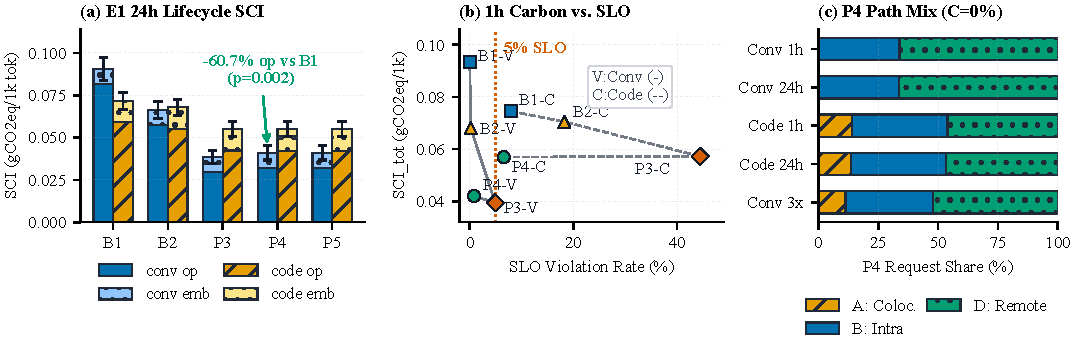
\includegraphics[width=\ifdefined\BUILDELSEVIER 0.94\textwidth\else 0.58\textwidth\fi]{figures/fig5_e1_pareto_paths.pdf}
    \caption{Experiment \texttt{E1} cluster evaluation ($N=10$ seeds, 95\% Student-$t$ CIs): (a) 24h operational plus embodied SCI; (b) 1h carbon--SLO frontier against the 5\% boundary; (c) adaptive \texttt{P4} path mix showing Path C pruned to 0\% at 10~Gbps WAN.}
    \label{fig:e1_pareto}
\end{figure*}

\begin{table*}[t]
\centering
\caption{Experiment \texttt{E1} Multi-Region Cluster Metrics (Mean $\pm$ 95\% CI, $N=10$ Seeds; Paired vs.\ \texttt{P4})}
\label{tab:e1_results}
\scriptsize
\setlength{\tabcolsep}{2.6pt}
\ifdefined\BUILDELSEVIER\resizebox{\textwidth}{!}{\fi
\begin{tabular}{@{}llcccccc@{}}
\toprule
\textbf{Case} & \textbf{Policy} & $\textbf{SCI}_{\text{op}}$ \textbf{(g/1k)} & $\textbf{SCI}_{\text{tot}}$ \textbf{(g/1k)} & \textbf{TTFT P95 (ms)} & \textbf{SLO (\%)} & \textbf{Effect ($r_{\text{rb}}, p$)} & \textbf{Verdict (H1/H2)} \\
\midrule
1h Conv & \texttt{B1} (Coloc.) & $0.08431 \pm 0.00681$ & $0.09329 \pm 0.00681$ & $268.6 \pm 0.0$ & $0.0005 \pm 0.001$ & $-1.00, 0.002$ (op) & Baseline \\
1h Conv & \texttt{B2} (Intra P/D) & $0.05901 \pm 0.00472$ & $0.06799 \pm 0.00472$ & $300.3 \pm 0.2$ & $0.20 \pm 0.04$ & $-1.00, 0.002$ (op) & Baseline \\
1h Conv & \texttt{P3} (Uncond.) & $0.03040 \pm 0.00306$ & $0.03938 \pm 0.00306$ & $1062.3 \pm 136.1$ & $4.93 \pm 1.02$ & $-1.00, 0.002$ (SLO) & Tail Degrad. \\
1h Conv & \texttt{P4} (Hybrid) & $\mathbf{0.03307 \pm 0.00365}$ & $\mathbf{0.04205 \pm 0.00365}$ & $\mathbf{506.4 \pm 2.1}$ & $\mathbf{0.81 \pm 0.06}$ & \text{--} & \textbf{SUPPORTED} \\
\midrule
24h Conv & \texttt{B1} / \texttt{B2} & $0.08150$ / $0.05726$ & $0.09055$ / $0.06631$ & $268.6$ / $300.3$ & $0.00$ / $0.20$ & $-1.00, 0.002$ (op) & Baselines \\
24h Conv & \texttt{P3} (Uncond.) & $0.02953 \pm 0.00369$ & $0.03858 \pm 0.00371$ & $1190.4 \pm 156.0$ & $5.90 \pm 1.10$ & $-1.00, 0.002$ (SLO) & Breaches 5\% \\
24h Conv & \texttt{P4} (Hybrid) & $\mathbf{0.03203 \pm 0.00434}$ & $\mathbf{0.04108 \pm 0.00436}$ & $\mathbf{504.5 \pm 3.7}$ & $\mathbf{0.82 \pm 0.03}$ & \text{--} & \textbf{SUPPORTED} \\
\midrule
1h Code & \texttt{B1} / \texttt{B2} & $0.06182$ / $0.05773$ & $0.07457$ / $0.07048$ & $592.8$ / $3209.1$ & $7.91$ / $18.25$ & $-1.00, 0.002$ (op) & CV 13.15 \\
1h Code & \texttt{P3} (Uncond.) & $0.04441 \pm 0.00385$ & $0.05722 \pm 0.00385$ & $39317.8 \pm 793.9$ & $44.45 \pm 0.28$ & $-1.00, 0.002$ (SLO) & WAN Collapse \\
1h Code & \texttt{P4} (Hybrid) & $\mathbf{0.04419 \pm 0.00388}$ & $\mathbf{0.05694 \pm 0.00388}$ & $\mathbf{1613.8 \pm 4.3}$ & $\mathbf{6.57 \pm 0.25}$ & \text{--} & \textbf{H1 Part./H2 Sup.} \\
\midrule
24h Code & \texttt{B1}/\texttt{B2}/\texttt{P3} & $0.05911$/$0.05525$/$0.04235$ & $0.07171$/$0.06784$/$0.05495$ & $612.5$/$3380$/$30725$ & $8.46$/$19.47$/$44.57$ & $\le -0.82, \le 0.020$ & Baselines \\
24h Code & \texttt{P4} / \texttt{P5} & $\mathbf{0.04226}$ / $0.04226$ & $\mathbf{0.05485}$ / $0.05485$ & $\mathbf{1598.9}$ / $1599.0$ & $\mathbf{6.24}$ / $6.23$ & $|r_{\text{rb}}| \le 0.20, \ge 0.652$ & \textbf{H1 Part./H2 Sup.} \\
\bottomrule
\end{tabular}%
\ifdefined\BUILDELSEVIER}\fi
\end{table*}

Under bursty coding completions (\texttt{code}, $\text{CV}=13.152$, mean $2{,}047.8$-token prompts; Fig.~\ref{fig:e1_pareto}b), \texttt{P4} cuts $\text{SCI}_{\text{op}}$ by 28.51\% versus \texttt{B1} ($\Delta = -0.01763$ [1h], $-0.01685$ [24h], $d_z \in [-13.14, -9.73]$, $p = 0.002$) and 23.45\%--23.51\% versus \texttt{B2} ($p = 0.002$). Unconditional \texttt{P3} saturates the WAN with 192.5--193.1~GB/1k-req KV transfers, driving SLO violations to 44.45\%--44.57\% (TTFT P95 = 30.7--39.3~s). To trace where spatial gains originate, \texttt{P4}'s gates prune cross-region Path C cleanly to \textbf{0.00\%} at 10--25~Gbps (Section~\ref{subsec:res_sweeps}). Consequently, \texttt{P4}'s operational carbon reductions come primarily from \textbf{Path D} (whole-request remote clean-grid execution: 66.13\%--66.27\% on \texttt{conv}, 46.08\%--46.74\% on \texttt{code}) paired with local intra-DC fallbacks onto Path B (33.54\%--39.81\%) and Path A (0.20\%--14.11\%), cutting \texttt{P3}'s \texttt{code} SLO violations by 85.22\% (1h, $\Delta = -37.88\text{ pp}$ [-38.21, -37.55], $d_z = -82.83$, $p = 0.002$) and 86.01\% (24h, $\Delta = -38.34\text{ pp}$ [-38.57, -38.10], $d_z = -118.80$). Oracle 30-min grid lookahead \texttt{P5} matches \texttt{P4} within 0.02\% on carbon and 0.25\% on SLOs ($p \ge 0.160$).

\subsection{\texorpdfstring{E2 \& SW4}{E2 and SW4}: Serverless Keep-Alive and Loader Sensitivity}\label{subsec:res_e2}
Table~\ref{tab:e2_results} and Fig.~\ref{fig:e2_serverless} reveal an inverse regional trade-off for dynamic keep-alive (\texttt{S3}). On carbon-intensive \texttt{TEPCO} (581.6~gCO$_2$eq/kWh), 24h GapHazard \texttt{S3} achieves the lowest operational intensity ($\text{SCI}_{\text{op}}=0.10825$), trimming operational carbon by 8.05\% below scale-to-zero \texttt{S1} ($\Delta=-0.00948$ [-0.01058, -0.00838], $r_{\text{rb}}=-1.000$), 7.03\% below 30~s static \texttt{S2} ($\Delta=-0.00819$ [-0.00873, -0.00764]), and 11.02\% below 60~s \texttt{S2b} ($\Delta=-0.01340$, all $p=0.002$). However, aggressive dirty-slot eviction leaves 28.60\% SLO violations (4,529 cold starts) versus 19.45\% (\texttt{S2}) and 13.03\% (\texttt{S2b}), though well below \texttt{S1} (40.25\%), partially supporting \textbf{H3}.

\begin{figure*}[t]
    \centering
    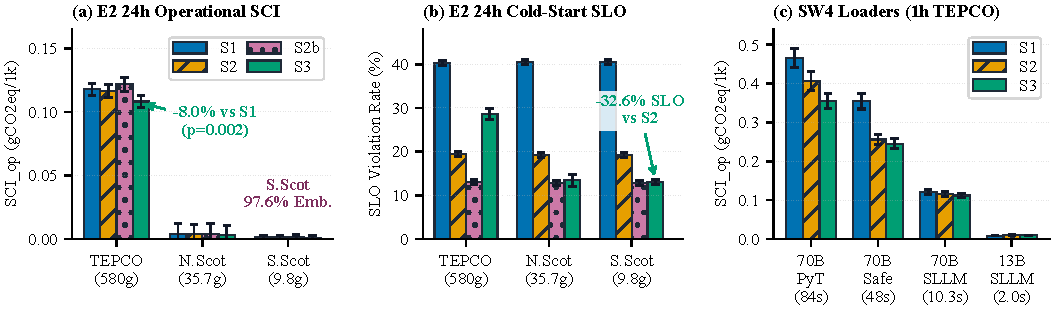
\includegraphics[width=\ifdefined\BUILDELSEVIER 0.94\textwidth\else 0.58\textwidth\fi]{figures/fig6_e2_serverless.pdf}
    \caption{Experiment \texttt{E2} and \texttt{SW4} serverless evaluation ($N=10$ seeds, 95\% CIs): (a) 24h operational SCI; (b) 24h cold-start SLO violations across grid intensities; (c) \texttt{SW4} loader sensitivity (84~s PyTorch down to 10.3~s ServerlessLLM and 2.0~s 13B).}
    \label{fig:e2_serverless}
\end{figure*}

\begin{table}[t]
\centering
\caption{Experiment \texttt{E2} 24h Serverless Keep-Alive Metrics ($N=10$ Seeds)}
\label{tab:e2_results}
\scriptsize
\setlength{\tabcolsep}{2.4pt}
\begin{tabular}{@{}llcccc@{}}
\toprule
\textbf{Region} & \textbf{Pol.} & $\textbf{SCI}_{\text{op}}$ & \textbf{Emb.\ (\%)} & \textbf{SLO (\%)} & \textbf{Cold Starts} \\
\midrule
\texttt{TEPCO} & \texttt{S1} ($0\text{ s}$) & $0.11773$ & $22.2$ & $40.25$ & $6{,}271.6$ \\
\texttt{TEPCO} & \texttt{S2} ($30\text{ s}$) & $0.11644$ & $22.4$ & $19.45$ & $3{,}054.7$ \\
\texttt{TEPCO} & \texttt{S2b} ($60\text{ s}$) & $0.12166$ & $21.6$ & $\mathbf{13.03}$ & $2{,}081.0$ \\
\texttt{TEPCO} & \texttt{S3} (GapHaz.) & $\mathbf{0.10825}$ & $23.7$ & $28.60$ & $4{,}529.0$ \\
\midrule
\texttt{N.\ Scot.} & \texttt{S1} ($0\text{ s}$) & $0.00373$ & $94.6$ & $40.48$ & $6{,}373.4$ \\
\texttt{N.\ Scot.} & \texttt{S2} ($30\text{ s}$) & $0.00362$ & $94.7$ & $19.29$ & $3{,}069.1$ \\
\texttt{N.\ Scot.} & \texttt{S2b} ($60\text{ s}$) & $0.00378$ & $94.6$ & $\mathbf{12.84}$ & $2{,}073.4$ \\
\texttt{N.\ Scot.} & \texttt{S3} (GapHaz.) & $\mathbf{0.00323}$ & $\mathbf{95.0}$ & $13.40$ & $2{,}164.8$ \\
\midrule
\texttt{S.\ Scot.} & \texttt{S1} ($0\text{ s}$) & $0.00106$ & $97.4$ & $40.48$ & $6{,}373.4$ \\
\texttt{S.\ Scot.} & \texttt{S2} ($30\text{ s}$) & $0.00103$ & $97.4$ & $19.29$ & $3{,}069.1$ \\
\texttt{S.\ Scot.} & \texttt{S2b} ($60\text{ s}$) & $0.00108$ & $97.4$ & $\mathbf{12.84}$ & $2{,}073.4$ \\
\texttt{S.\ Scot.} & \texttt{S3} (GapHaz.) & $\mathbf{0.00094}$ & $\mathbf{97.6}$ & $12.99$ & $2{,}098.4$ \\
\bottomrule
\end{tabular}
\end{table}

Conversely, on clean \texttt{South Scotland} (9.75~gCO$_2$eq/kWh), inverse intensity scaling in Eq.~\eqref{eq:gaphazard} extends warm retention during clean intervals, cutting cold-start SLO violations by \textbf{32.63\%} relative to 30~s \texttt{S2} ($\Delta = -6.29\text{ pp}$ [-6.60, -5.99], $12.99\%$ vs.\ $19.29\%$, $r_{\text{rb}}=-1.000$, $p=0.002$) while statistically tying 60~s \texttt{S2b} ($12.84\%$, $p=0.125$) at numerically lower $\text{SCI}_{\text{op}}$ ($0.00094$, $p=0.084$ vs.\ \texttt{S1}/\texttt{S2}). Embodied hardware accounts for 97.4\%--97.6\% of clean-grid lifecycle SCI ($\text{SCI}_{\text{emb}}=0.03308$), supporting \textbf{H4}. Volatile \texttt{North Scotland} displays zero-carbon wind slots that erase operational differences ($p \ge 0.50$) while retaining the -30.50\% SLO reduction versus \texttt{S2} ($\Delta=-5.88\text{ pp}$, $p=0.002$).

In \texttt{SW4} (1h \texttt{TEPCO}, Fig.~\ref{fig:e2_serverless}c), slow 70B loaders amplify \texttt{S3} operational carbon savings: -23.74\% vs.\ \texttt{S1} under PyTorch ($0.46686 \rightarrow 0.35601$ at 84~s) and -30.93\% under Safetensors ($0.35452 \rightarrow 0.24488$ at 48~s), whereas fast \texttt{opt\_13b} (2.0~s) favors \texttt{S1} on carbon (0.00831 vs.\ 0.00936) at 16.02\% vs.\ 3.60\% SLO violations. Replacing the 20\% idle ratio with H100's 8.6\% hardware idle ratio (60~W/700~W) cuts \texttt{S3} $\text{SCI}_{\text{op}}$ by another 14.43\% ($0.11193 \rightarrow 0.09578$).

\subsection{Sensitivity Sweeps (\texorpdfstring{\texttt{SW1--SW3}}{SW1-SW3}) and Clean Scale-Out Paradox (\texorpdfstring{\texttt{H4}}{H4})}\label{subsec:res_sweeps}
Fig.~\ref{fig:sw_paradox} and Table~\ref{tab:wan_pathmix} expose regime boundaries across load, WAN bandwidth, hardware tiering, and cluster capacity:
\begin{enumerate}
    \item \textbf{SW1 Load Scaling (0.5x--3.0x conv):} At 3.0x load, \texttt{P3} saturates clean pools (71.94\% SLO viol., TTFT P95 = 446.7~s), \texttt{B1} stalls via colocation (54.48\% viol., TPOT P95 = 2,331~ms), and \texttt{B2} reaches 20.00\%. Activating 11.30\% Path A local spillover with Path B (36.62\%) and Path D (52.08\%), \texttt{P4} holds 2.89\% violations ($\text{SCI}_{\text{op}}=0.03483$ vs.\ \texttt{B1} 0.04943).
    \item \textbf{SW2 Grid \& Forecast Noise:} UK NESO forecasts, 30--60~min lags, and $2\times$ noise shift \texttt{P4} $\text{SCI}_{\text{tot}}$ by $<0.3\%$. Across a low-differential UK pair (\texttt{South Scotland} + \texttt{North West England}), \texttt{P4} holds 0.08\% violations ($\text{SCI}_{\text{op}}=0.00513$) vs.\ \texttt{P3}'s 10.71\% (0.00425).
    \item \textbf{SW3 Hardware Tiers \& WAN Path Mix:} Under \texttt{L4} decode nodes, \texttt{B2} (24.73\%) and \texttt{P3} (53.47\%) suffer decode SLO collapse, whereas \texttt{P4} holds 0.76\% violations (Fig.~\ref{fig:sw_paradox}b). Table~\ref{tab:wan_pathmix} explains WAN insensitivity: raising WAN bandwidth from 10 to 100~Gbps halves \texttt{P3}'s \texttt{code} violations from 44.45\% to 20.78\% (and high-rate 2.0x \texttt{conv} from 42.20\% to 3.76\%), whereas \texttt{P4} keeps Path C pruned (\textbf{0.00\%} at 10--25~Gbps; 0.02\% at 100~Gbps \texttt{conv}) because clean-region whole-request routing (Path D: 46.08\% \texttt{code}, 62.97\% \texttt{conv}) and local disaggregation (Path B) dominate cross-region KV pipelining under 20--200~ms RTT. Under a strict 125~ms TTFT cap (\texttt{strict\_code}), every fixed-capacity policy exceeds 5\% (\texttt{P4} 48.69\%, \texttt{B1} 53.30\%).
    \item \textbf{H4 Clean Scale-Out Paradox:} Across 24h \texttt{E1}, clean \texttt{South Scotland} reaches 93.0\% embodied share on \texttt{code} (90.7\% on \texttt{conv}). On all-UK nodes (where balanced \texttt{P4\_equal} carries a 53.3\% embodied share), adding four spare clean nodes (\texttt{P3\_overprov\_plus4}, 10 vs.\ 6 nodes) trims $\text{SCI}_{\text{op}}$ by only -3.94\% ($0.00804$ vs.\ $0.00837$) while inflating net lifecycle $\text{SCI}_{\text{tot}}$ by \textbf{+32.61\%} under 4-year uniform amortization ($0.02300$ vs.\ $0.01735$) and \textbf{+27.71\%} under decoupled 9~yr host / 3~yr GPU lifetimes ($0.01937$ vs.\ $0.01516$, Fig.~\ref{fig:sw_paradox}c), supporting \textbf{H4}.
\end{enumerate}

\begin{table}[t]
\centering
\caption{WAN Bandwidth Sweep (\texttt{SW3c}) Path Mix and Performance ($N=10$ Seeds)}
\label{tab:wan_pathmix}
\scriptsize
\setlength{\tabcolsep}{2.1pt}
\begin{tabular}{@{}lllccccccc@{}}
\toprule
\textbf{Work.} & \textbf{BW} & \textbf{Pol.} & $\textbf{SCI}_{\text{op}}$ & \textbf{SLO} & \textbf{P95 (ms)} & \textbf{A} & \textbf{B} & \textbf{C} & \textbf{D (\%)} \\
\midrule
\texttt{code} & 10G & \texttt{P3} & 0.04441 & 44.45\% & 39,318 & 0.0 & 56.6 & 43.4 & 0.0 \\
\texttt{code} & 10G & \texttt{P4} & 0.04419 & \textbf{6.57\%} & \textbf{1,614} & 14.1 & 39.8 & \textbf{0.0} & \textbf{46.1} \\
\texttt{code} & 25G & \texttt{P3} & 0.04403 & 32.12\% & 7,110 & 0.0 & 56.7 & 43.3 & 0.0 \\
\texttt{code} & 100G & \texttt{P3} & 0.04391 & 20.78\% & 3,341 & 0.0 & 56.7 & 43.3 & 0.0 \\
\texttt{code} & 100G & \texttt{P4} & 0.04419 & \textbf{6.57\%} & \textbf{1,614} & 14.1 & 39.8 & \textbf{0.0} & \textbf{46.1} \\
\midrule
\texttt{conv} 2x & 10G & \texttt{P3} & 0.02481 & 42.20\% & 162,595 & 0.0 & 49.8 & 50.2 & 0.0 \\
\texttt{conv} 2x & 10G & \texttt{P4} & 0.03191 & \textbf{1.10\%} & \textbf{881} & 1.6 & 35.5 & \textbf{0.0} & \textbf{63.0} \\
\texttt{conv} 2x & 25G & \texttt{P3} & 0.02502 & 9.63\% & 1,694 & 0.0 & 49.1 & 50.9 & 0.0 \\
\texttt{conv} 2x & 100G & \texttt{P3} & 0.02488 & 3.76\% & 1,492 & 0.0 & 49.5 & 50.5 & 0.0 \\
\texttt{conv} 2x & 100G & \texttt{P4} & 0.03193 & \textbf{1.10\%} & \textbf{881} & 1.6 & 35.4 & \textbf{0.02} & \textbf{63.0} \\
\bottomrule
\end{tabular}
\end{table}

\begin{figure*}[t]
    \centering
    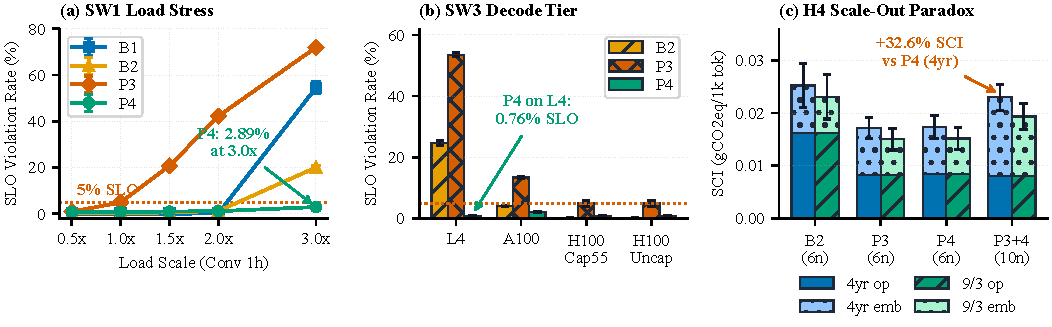
\includegraphics[width=\ifdefined\BUILDELSEVIER 0.94\textwidth\else 0.57\textwidth\fi]{figures/fig7_sw_sensitivity_embodied.pdf}
    \caption{Robustness and lifecycle evaluations ($N=10$ seeds, 95\% CIs): (a) \texttt{SW1} load scaling (\texttt{P4} holds 2.89\% at 3.0x); (b) \texttt{SW3} decode GPU tiers (\texttt{P4} holds 0.76\% on \texttt{L4}); (c) \texttt{H4} clean over-provisioning (+4 nodes) raising net $\text{SCI}_{\text{tot}}$ by +27.71\% to +32.61\%.}
    \label{fig:sw_paradox}
\end{figure*}

\subsection{Summary Answers to Research Questions (\texorpdfstring{\texttt{RQ1--RQ4}}{RQ1-RQ4})}\label{subsec:rq_answers}
\begin{itemize}
    \item \textbf{RQ1:} While GreenLLM~\cite{shi2024greenllm} handles single-cluster P/D carbon and multi-DC routers~\cite{topcu2026tension,moore2025slit,zhang2026context,bernhard2026cleanest} schedule colocated LLMs, 75.4\% of 61 works omit embodied carbon, 0/8 geo-routers use P/D or WAN KV gating, and 0 implemented systems unify all four axes with keep-alive.
    \item \textbf{RQ2:} Hybrid routing (\texttt{P4}) cuts \texttt{conv} $\text{SCI}_{\text{op}}$ by 60.70\%--60.77\% ($\text{SCI}_{\text{tot}}$ 54.64\%--54.92\%, $|r_{\text{rb}}|=1.000$) at $<1\%$ SLO violation and trims \texttt{P3} \texttt{code} SLO violations by 85.22\%--86.01\% by pruning Path C (0\%) to rely on Path D and local fallbacks.
    \item \textbf{RQ3:} GapHazard (\texttt{S3}) saves 7.03\%--11.02\% \texttt{TEPCO} $\text{SCI}_{\text{op}}$ (23.74\%--30.93\% for 48--84~s loaders) with 28.60\% SLO violations, yet flips to cut clean \texttt{South Scotland} SLO violations by 32.63\% vs.\ 30~s TTL.
    \item \textbf{RQ4:} Embodied carbon hits 93.0\%--97.6\% of clean-grid SCI, so four spare clean nodes raise net $\text{SCI}_{\text{tot}}$ by +32.61\% (4-yr) and +27.71\% (9~yr/3~yr).
\end{itemize}
